\documentclass{article}
\usepackage{ctex}
\usepackage{amsmath}
\usepackage{graphicx}
\usepackage{wrapfig}
\usepackage{caption}
\usepackage[top=0.8in, bottom=0.8in,left=0.8in, right=0.8in]{geometry}
\usepackage{float} 
\usepackage{subfigure}
\usepackage{subcaption}
\usepackage{bm}
\xeCJKsetup{CJKmath=true} 

\begin{document}
\section*{悬链线(40分)}
\begin{wrapfigure}{r}{7cm}
	\vspace{-15pt}    % 对应高度1
	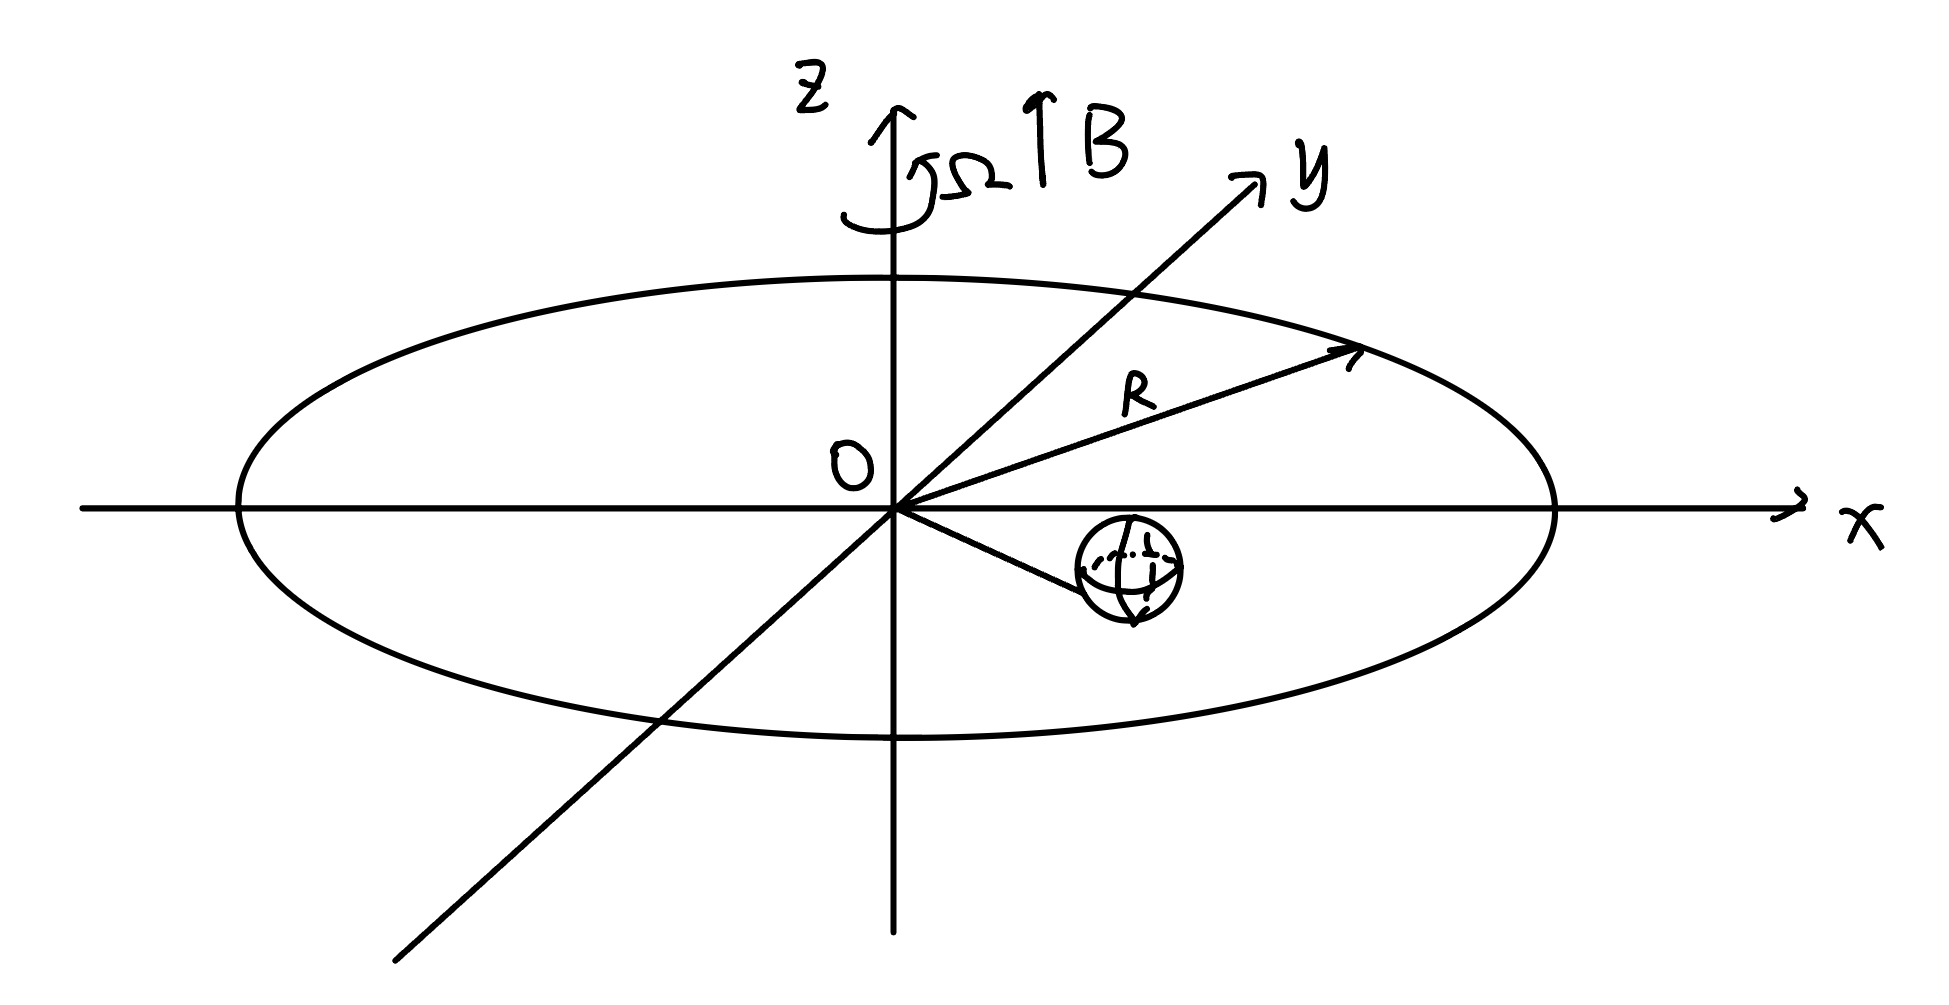
\includegraphics[width=7cm]{img/1.jpeg}\\
	\vspace{-15pt}    % 对应高度2
	\caption{}
	\vspace{-15pt}    % 对应高度3
\end{wrapfigure}
竖直平面内挂有一根柔软的质量线密度为$\lambda$的均匀导线,其中通有电流$I$,存在如图所示的匀强磁场$B$,重力场$g$
已知底部$(x,y)=(0,0)$处张力为$T_0$。
试求其形状的微分方程,用$\mathrm{d}x,\mathrm{d}y$表示
\begin{itemize}
\item[(1)]取$B=0$,求其轨迹方程。\par
    注:双曲函数定义
    $$
    \cosh(x)=\dfrac{\mathrm{e}^{x}+\mathrm{e}^{-x}}{2},\sinh(\theta)=\dfrac{\mathrm{e}^{x}-\mathrm{e}^{-x}}{2}
    $$
\item[(2)]取$g=0$,求其轨迹方程。
\item[(3)]试求其形状的微分方程,用$\mathrm{d}x,\mathrm{d}y$表示.  
\end{itemize}
\end{document}